\section{Introduction}

In order to make use of the Manhattan world assumption we must first
discover the orientation of the Manhattan world with respect to the
camera. Equivalent to the Manhattan world assumption is the statement
that there exists a ``canonical'' coordinate frame in which world
surfaces are axis--aligned. The topic of this chapter is the
estimation of $\SceneR$ from a sequence of input images. As described
in preceeding chapters, we assume a structure--from--motion system
providing a continuous estimate of the camera pose. We will not use
any point cloud generated from structure--from--motion in this
chapter.

$\SceneR$ is constant for all frames since the structure--from--motion
system measures consecutive poses with respect to single global
coordinate frame.

The problem of determining $\SceneR$ in the conext of a single image
is equivalent to the problem of vanishing point detection since three
vanishing points and a calibrated camera give $\SceneR$ in closed
form, and vice--versa. TODO: give equations here? Therefore the
algorithms presented in this chapter may be viewed as a generalization
of vanishing point detection to multiple calibrated views.

TODO: note on point estimate of R rather than joint inference.

\section{Background}

\subsection{Single View}

Several approaches to single--image vanishing point detection have
been proposed in the literature
\cite{Barnard83,Zhang02,Shufelt99}. Common among all such approaches
is the use of line segments as the fundamental observation from which
inference is performed. Each of the vanishing points under
consideration are assumed to generate several assocated line segments,
all of which meet at the vanishing point (modulo measurement errors of
course). The actual estimation of vanishing points is approached in
various ways. The classic approach due to Barnard \cite{Barnard83} was
to project images onto the Gaussian sphere and use the Hough transform
to identify vanishing points. Several authors have proposed similar
voting schemes under different parametrisations of the accumulator
space that improve statistical robustness \cite{Brillaut91}.

Shufelt introduced explicit error models for observed line segments
\cite{Shufelt99}, but retained the voting--based estimation
strategy. Hartley and Zisserman \cite{Hartley00} first proposed a
generative model relating vanishing point to line segments and cast
maximum likelihood estimation as a non--linear estimation problem. We
make these exact probabilistic assumptions in the present
work. Kanatani \cite{Kanatani93} minimized the algebraic deviation of
the vanishing point from observed line segments, which leads to an
efficient linear least--squares solution at the cost of a less precise
error model. Schinder and Dellaert \cite{Schindler04} laid out an
integrated Bayesian approach to the estimation of multiple vanishing
points.

The approaches discussed thus far estimate vanishing points
independently, using K--means clustering or the expectation
maximisation algorithm to resolve the assignment of line segments to
vanishing points. Coughlan and Yuille \cite{Coughlan99} observed that
under the Manhattan world assumption the three cardinal vanishing
points are mutually orthogonal and hence their locations in the image
plane are highly correlated. Rather than estimating three independent
vanishing points, the authors cast the estimation problems in terms of
Euler angles corresponding to $\SceneR$, resulting in a three--DoF
estimation problem in place of the 6 for independent vanishing point
estimation. Koseck\`{a} and Zhang \cite{Zhang02} showed that the
Manhattan world assumption can be exploited even in the case of an
uncalbirated camera. Their approach used a prior on camera intrinsics
to condition the estimation process, though the estimation of three
vanishing points was not explicitly coupled after this stage.

Denis \etal \cite{Denis08} took this a step further by exploiting a
prior on the rotation $\SceneR$ learned from training data. Whereas
Coughland and Yuille used a discretization of the space of rotations
to identify $\SceneR$, they showed how to exploit the Manhattan world
assumption under the more principled Expectation--Maximization
approach of Schindler and Dellaert. The M--step in their approach is a
non--linear optimization over rotations, leveraging the genuine
maximum likelihood reprojection error of Hartley and Zisserman.

Just when it seemed that vanishing point detection had reached the
pinnacle of pure, relentlessly uncompromising Bayesian inference,
Mirzaei and Roumeliotis \cite{Mirzaei11} showed that the estimation
can be solved globally and in closed form using an off--the--shelf
polynomial solver. Their approach assumes the algebraic error and it
is not clear whether the reprojection error leads to a likelihood that
is amenable to a polynomial solution. We discuss these ideas further
in the last section of this chapter.

\subsection{Mulitple Views}

The literature concerning multiple views leverage different approaches
to recover $\SceneR$. Furukawa and Curless \cite{Furukawa09} use
multiple--view stereo to recover a dense point cloud, then estimate
$\SceneR$ by clustering surface normals on the unit hemisphere.

Werner and Zisserman \cite{Werner02} identify vanishing points
independently in several uncalibrated views, then resolve associations
between views using a simple combinatorial search.

\section{Overview of Proposed Approach}

Reliable vanishing point detection from single images is fundamentally
challenging in environments in which axis--oriented edges are rare, or
in which one or two cardinal orientations have very few associated
edges. Both scenarios are common in video sequences of indoor
environments since the camera often views only a small portion of the
scene. On the other hand, obtaining a dense reconstruction is a
complex and computationally expensive pre--requisite for a
three--parameter estimation problem. Furthermore, the point cloud
provided by on--line structure--from--motion is too sparse to obtain
accurate surface normal estimates.

We overcome these limitations by reasoning directly in terms of line
segments and integrating observations from many frames into the
estimation. Since $\SceneR$ is fixed for all frames it makes sense to
leverage all available data during estimation. Whereas previous
approaches often estimate vanishing points as a precursor to
reconstructing camera poses \cite{Zhang02,Werner02}, we prefer to rely
on a vanishing point--less structure--from--motion system to provide
camera poses, then recover vanishing points afterwards. Under this
problem setup we can relate line segments in all views directly to
$\SceneR$ and therefore to perform full joint estimation. We show that
this is both computationally efficient and avoids the fragile
single--view estimation scenario.

\section{Generative Model}

\begin{figure}[tb]
  \centering
  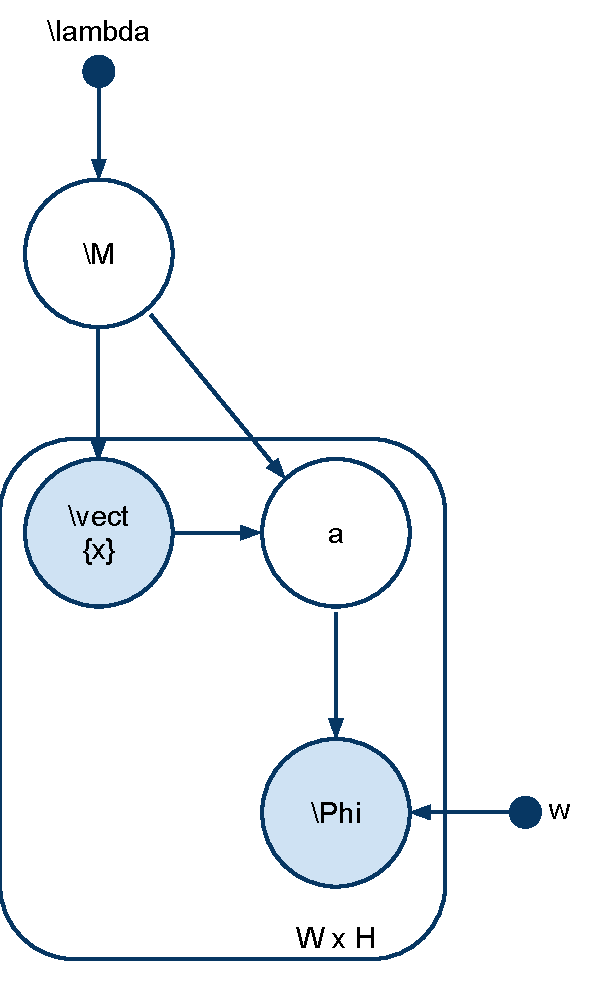
\includegraphics[width=0.3\textwidth]{graphical-model}
  \caption{A graphical model relating line segments to vanishing
    points.}
  \label{fig:R-graphical}
\end{figure}

\begin{figure}[tb]
  \centering
  \includegraphics[width=0.5\textwidth]{line-sampling}
  \caption{Illustration of our error model for line segments.}
  \label{fig:line-sampling}
\end{figure}

We assume the graphical model shown in \figref{R-graphical}. The
variable $\Indicator$ bears special explanation. It is a binary vector
of length 4 indicating which vanishing point the $i$\th line segment
is associated with. Exactly one element is set to 1, the remainder are
0. The first three elements correspond to the three vanishing points;
the fourth element corresponds to a spurious observation not
associated with any of the three Manhattan directions. We denote
the (binary) value of one of the components by $\Indicator_{ik}$ but
we will also write $\Indicator_i=k$ as shorthand for the event that
$\Indicator_i$ is the binary vector with the $k$\th element set to 1
and the others set to zero. For clarity we write
$\Indicator_i=\Spurious$ in place of $\Indicator_i=4$.

The generative process operates as follows. First we sample a scene
orientation $\SceneR$ and the rotation component of the camera pose
for each frame. Camera translation plays no part when reasoning about
vanishing points, which are at infinity. Next we sample a series of
indicators and line segments. First we sample $\Indicator_i$ from a
categorical distribution with mixing parameters $\Mixing$. Next, if
$\Indicator_i=\Spurious$ then the line segment $\TrueSeg$ is sampled
uniformly from the image. Otherwise, we sample $\TrueSeg$ as follows.

The vanishing point $\vpt$ corresponding to $\Indicator_i$ is
\begin{equation}
  \vpt_{\Indicator_i} = \CamR_i \SceneR \ebasis_{\Indicator_i} ~.
\end{equation}
We sample a ray through $\vpt$, then sample a line segment $\TrueSeg =
(\TrueStartPt,\TrueEndPt)$ along the ray. Finally we sample Gaussian
noise to arrive at the measured line segment
$\LineSeg=(\StartPt,\EndPt)$:
\begin{eqnarray}
  \StartPt &\sim& \NormalDistr(\TrueStartPt, \Sigma) \\
  \EndPt &\sim& \NormalDistr(\TrueEndPt, \Sigma) ~.
\end{eqnarray}
This is illustated in \figref{R-graphical}.

\subsection{Likelihood for Line Segments}

The likelihood $P(\LineSeg_i ~|~ \Indicator_i,\SceneR)$ can be
simplified as follows
\begin{eqnarray}
  P(\LineSeg_i ~|~ \Indicator_i,\SceneR) &=& 
  \int
    P(\LineSeg_i ~|~ \TrueSeg)
    ~ P(\TrueSeg ~|~ \Indicator_i,\SceneR)
  ~\intd \TrueSeg \\
  &=&
    \NormalDistr(\dist(\LineSeg)_i,\vpt_{\Indicator_i}); 0, \sigma)
\end{eqnarray}
where $\dist(\LineSeg,\vpt)$ is the reprojection error illustrated in
\figref{reprojection-error}. $\dist$ is computed as follows. First,
cast a line between the vanishing point $\vpt$ and the mid--point of
the line segment $\LineSeg$,
\begin{equation}
  \ReprojLine_{ik} =
    \vpt_k \cross \frac{\StartPt_i+\EndPt_i}{2}
\end{equation}
Now, $\dist$ is the distance between the line $\ReprojLine$ and either
end point of $\LineSeg$ (the two quantities are equal, as evident by
inspecting \figref{reprojection-error}). So
\begin{eqnarray}
  \dist(\LineSeg_i,\vpt_k) &=& 
  \frac
    {\StartPt_i \cdot \ReprojLine_{ik}}
    {(\StartPt_{i}\cdot\ez) \eta_{ik}}\\
  \eta_{ik} &=&
   \sqrt{(\ReprojLine_{ik} \cdot \ex)^2 +
         (\ReprojLine_{ik} \cdot \ey)^2}
  ~.
\end{eqnarray}

\begin{figure}[tb]
  \centering
  \includegraphics[width=0.5\textwidth]{reprojection-error}
  \caption{Illustration of the reprojection error.}
  \label{fig:reprojection-error}
\end{figure}

\subsection{Complete Data Likelihood}

In sections to follow we will need to deal with the so--called
complete data likelihood,
\begin{equation}
  P(\LineSegs,\Indicators ~|~ \SceneR) =
    \prod_i P(\LineSeg_i,\Indicator_i ~|~ \SceneR)
\end{equation}

The likelihood terms $P(\LineSeg_i,\Indicator_i ~|~ \SceneR)$ depends
on the $\Indicator_i$ in a complicated way, since $\LineSeg_i$ is
drawn from completely different distributions depending on its value:
\begin{equation}
  P(\LineSeg_i,\Indicator_i ~|~ \SceneR) =
  \begin{cases}
    \Mixing_1 
    \NormalDistr\bigr(\dist(\LineSeg_i, \CamR_i\SceneR\ex\bigl); 0,\sigma),
      & \mbox{if } \Indicator_i = 1 \\
    \Mixing_2
    \NormalDistr\bigr(\dist(\LineSeg_i, \CamR_i\SceneR\ey\bigl); 0,\sigma),
      & \mbox{if } \Indicator_i = 2 \\
    \Mixing_3
    \NormalDistr\bigr(\dist(\LineSeg_i, \CamR_i\SceneR\ez\bigl); 0,\sigma),
      & \mbox{if } \Indicator_i = 3 \\
    \Mixing_{\Spurious},
      & \mbox{if } \Indicator_i = \Spurious ~.
  \end{cases}
\end{equation}
Through our definition of $\Indicator_i$ as a binary vector we can
express this likelihood in the following analytic form,
\begin{equation}
  \label{eq:complete-likelihood}
  P(\LineSeg_i,\Indicator_i ~|~ \SceneR) =
  \prod_{k=1}^4 \Bigl( 
    P(\LineSeg_i ~|~ \Indicator_i=k,\SceneR)
    P(\Indicator_i=k ~|~ \SceneR)
  \Bigr)^{\Indicator_{ik}}
\end{equation}

\section{Inference}

\subsection{Detecting Line Segments}

We begin by running the Canny edge detector \cite{Canny86}, followed
by an edge linking algorithm \cite{Zhang02} to identify a set of
straight line segments $\LineSeg_j = \{\Pixel : \LineSeg_j\cdot\Pixel
= 0\}$.

\subsection{Estimating the Manhattan Coordinate Frame}

Under the model presented in the previous section, the
likelihood of $\SceneR$ is
\begin{equation}
  P(\LineSegs ~|~ \SceneR,\{\CamR_i\}) =
    \int P(\LineSegs,\Indicators ~|~ \SceneR,\{\CamR_i\})
    ~\intd\Indicators ~.
\end{equation}
For brevity we will omit the camera poses $\{\CamR_i\}$ in the
remainder of this section; it may be assumed that all probabilities
to follow are conditioned on $\{\CamR_i\}$.

The indicators $\Indicators$ are latent variables over which we need
to marginalize in order to perform inference on $\SceneR$. Integrating
explicitly over $\Indicator$ is intractible so we turn to the
Expectation--Maximization algorithm, which alternately refines
estimates of the posterior on $\Indicators$ (the ``E--step'') and
$\SceneR$ (the ``M--step'').

Due to the iterative nature of the EM algorithm we adopt superscript
notation for the scene rotation and indicators to make clear the
dependence between successive time steps. $\SceneR^t$ is the estimate
of the scene rotation at time $t$ and $\PosteriorEst^t$ is the
estimate for the posterior on $\Indicators$ at time $t$. We will treat
$\PosteriorEst$ as a continuous function, though of course behind the
scenes we are really just estimating sufficient statistics for
$\PosteriorEst$. Also note that we never actually store or estimate
the values of the indicators $\Indicators$, so we have no need for
superscripts on this variable. Although $\Indicator$ does appear in
the derivations to follow, in every equation we are either
marginalizing it out, or defining a function over it.

\subsubsection{The E--step}

In this phase we compute sufficient statistics for the posterior on
the indicators,
\begin{eqnarray}
  \PosteriorEst^t(\Indicators) &=&
    P(\Indicators ~|~ \LineSegs,\SceneR^t) \\
  \label{eq:posterior-est}
  &=&
    \frac{
      \prod_i P(\LineSeg_i,\Indicator_i ~|~\SceneR^t)
    }{
      \int \prod_i P(\LineSeg_i,\Indicator_i ~|~ \SceneR^t)
      ~\intd\Indicators
    }\\
\end{eqnarray}
Consider the term on the top line,
\begin{equation}
  P(\LineSeg_i,\Indicator_i ~|~\SceneR^t)
  =
  P(\LineSeg_i ~|~ \Indicator_i,\SceneR^t)
  P(\Indicator_i ~|~ \SceneR^t)
\end{equation}
As a function of $\Indicator_i$ this is simply a categorical
distribution, and since equation \eqnref{posterior-est} is a
normalized concatenation of categorical distributions, it is
itself a categorical distribution, meaning that the sufficient
statistics for $\PosteriorEst^t$ are nothing more than the
expectations
\begin{eqnarray}
  \Expected_{\PosteriorEst^t}\bigl[ \Indicator_{ik} \bigr]
  &=& 
    \int \Indicator_{ik} \PosteriorEst^t(\Indicators) ~\intd\Indicators \\
  &=& 
    \sum_{\Indicator_{ik}\in\{0,1\}}
    \Indicator_{ik} P(\Indicator_{ik} ~|~ \LineSeg_i, \SceneR^t)\\
  &=&
    P(\Indicator_i=k ~|~ \LineSeg_i, \SceneR^t)\\
  &=&
    \label{eq:expected-zik}
    \frac
        {P( \LineSeg_i, \Indicator_i=k ~|~ \SceneR^t)}
        {\sum_{j=0}^4 P(\LineSeg_i, \Indicator_i=j ~|~ \SceneR^t)}
\end{eqnarray}
where in the third line we have expanded the sum over the two possible
values for $\Indicator_{ik}$ and cancelled the one in which
$\Indicator_{ik}$ is 0. Substituting the specific forms for the the
complete data likelihood \eqnref{complete-likelihood},
\begin{eqnarray}
  \Expected_{\PosteriorEst^t}\bigl[ \Indicator_{ik} \bigr] 
  &=&
  \frac{
    \prod_{k=1}^4\limits \Bigl( 
      P(\LineSeg_i ~|~ \Indicator_i=k,\SceneR^t)
      P(\Indicator_i=k ~|~ \SceneR^t)
    \Bigr)^{\Indicator_{ik}}
  }{
    \sum_{\Indicator_i=1}^4\limits
    \prod_{k=1}^4\limits \Bigl( 
      P(\LineSeg_i ~|~ \Indicator_i=k,\SceneR^t)
      P(\Indicator_i=k ~|~ \SceneR^t)
    \Bigr)^{\Indicator_{ik}}
  }\\
  \label{eq:big-expectation}
  &=&
  \frac{
    \Bigl(
      \Mixing_{\Spurious}
      P(\LineSeg_i ~|~ \Indicator_i=\Spurious,\SceneR^t)
    \Bigr)^{\Indicator_{ik}}
    \prod_{k=1}^3\limits \Bigl(
      \Mixing_k
      P(\LineSeg_i ~|~ \Indicator_i=k,\SceneR^t)
    \Bigr)^{\Indicator_{ik}}
  }{
    \sum_{\Indicator_i=1}^4\limits \Biggl[
    \Bigl(
      \Mixing_{\Spurious}
      P(\LineSeg_i ~|~ \Indicator_i=\Spurious,\SceneR^t)
    \Bigr)^{\Indicator_{ik}}
    \prod_{k=1}^3\limits \Bigl( 
      \Mixing_k
      P(\LineSeg_i ~|~ \Indicator_i=k,\SceneR^t)
    \Bigr)^{\Indicator_{ik}}
    \Biggr]
  }
\end{eqnarray}
Substituting
\begin{eqnarray}
  \SpurJoint_i &=& 
    \Mixing_{\Spurious}
    P(\LineSeg_i ~|~ \Indicator_i=\Spurious,\SceneR^t) \\
  \SpurIndicator_i &=&
    \begin{cases}
      1, & \mbox{if } \Indicator_i = \Spurious \\
      0, & \mbox{otherwise}
    \end{cases}\\
\end{eqnarray}
into \eqnref{big-expectation} we have
\begin{eqnarray}
  \Expected_{\PosteriorEst^t}\bigl[ \Indicator_{ik} \bigr]
  &=&
  \frac{
    \SpurJoint_i^{\SpurIndicator_i}
    \Bigl(
      \Mixing_{\Indicator_i}
      \NormalDistr(\dist(\LineSeg,\CamR_i\SceneR^t\ebasis_k); 0, \sigma)
    \Bigr)^{1-\SpurIndicator_i}
  }{
    \sum_{\Indicator_i=1}^4\limits
    \SpurJoint_i^{\SpurIndicator_i}
    \Bigl(
      \Mixing_{\Indicator_i}
      \NormalDistr(\dist(\LineSeg,\CamR_i\SceneR^t\ebasis_{\Indicator_i}); 0, \sigma)
    \Bigr)^{1-\SpurIndicator_i}
  }\\
  &=&
  \frac{
    \SpurJoint_i^{\SpurIndicator_i}
    \Bigl(
      \Mixing_{\Indicator_i}
      \NormalDistr(\dist(\LineSeg,\CamR_i\SceneR^t\ebasis_k); 0, \sigma)
    \Bigr)^{1-\SpurIndicator_i}
  }{
    \SpurJoint_i +
    \sum_{\Indicator_i=1}^3\limits
    \Bigl(
      \Mixing_{\Indicator_i}
      \NormalDistr(\dist(\LineSeg,\CamR_i\SceneR^t\ebasis_{\Indicator_i}); 0, \sigma)
    \Bigr)
  }~.
\end{eqnarray}
Clearly the expression above can be evaluated for each indicator in
constant time, leading to a complexity for the E--step linear
in the number of observed line segments.

\subsubsection{M--step}

In the M--step we maximize the expectation of the complete data
log--likelihood with respect to the distribution
$\PosteriorEst^t$. The complete data log--likelihood is
\begin{equation}
  \label{eq:complete-loglikelihood}
  \log P(\LineSegs,\Indicators ~|~ \SceneR^t) =
  \sum_i \log P(\LineSeg_i,\Indicator_i ~|~ \SceneR^t) ~.
\end{equation}
Substituting \eqnref{complete-likelihood} gives
\begin{eqnarray}
  \log P(\LineSegs,\Indicators ~|~ \SceneR^t) 
  &=&
  \sum_i \sum_{k=1}^4 \Indicator_{ik} \Bigl(
    \log P(\LineSeg_i ~|~ \Indicator_i=k, \SceneR^t)
    + \log P(\Indicator_i=k ~|~ \SceneR^t)
  \Bigr)\\
  &=&
  \sum_i \sum_{k=1}^4 \Indicator_{ik} 
  \Bigl(
    \log \NormalDistr(\dist(\LineSeg_i, \CamR_i\SceneR^t\ebasis_k);0,\sigma)
    + \log \Mixing_k
  \Bigr)\\
  &=&
  \sum_i \sum_{k=1}^4 \Indicator_{ik} 
  \Bigl(
    \frac{\dist(\LineSeg_i, \CamR_i\SceneR^t\ebasis_k)^2}{2\sigma^2}
    + \log \Mixing_k
  \Bigr) + c\\
\end{eqnarray}
where $c$ is a constant arising from the logarithm of the constant
factor in the normal distribution, which we now drop since it plays no
part in the maximization to follow.

The expectation of the above with respect to the distribution
$\PosteriorEst^t$ is
\begin{eqnarray}
  \Expected_{\PosteriorEst^t}\Bigl[
    \log P(\LineSegs,\Indicators ~|~ \SceneR) 
  \Bigr]
  &=&
  \sum_i \sum_{k=1}^4
  \Expected_{\PosteriorEst^t} \bigl[ \Indicator_{ik} \bigr]
  \Bigl(
    \frac{-\dist(\LineSeg_i, \CamR_i\SceneR\ebasis_k)^2}{2\sigma^2}
    + \log \Mixing_k
  \Bigr)\\
  &=&
  \label{eq:expected-lik}
  \sum_i \sum_{k=1}^4
  \Resp_{ik}^t
  \Bigl(
    \frac{-\dist(\LineSeg_i, \CamR_i\SceneR\ebasis_k)^2}{2\sigma^2}
    + \log \Mixing_k
  \Bigr)
\end{eqnarray}
where in the last line we have defined and substituted
\begin{equation}
  \Resp_{ik}^t = 
  \Expected_{\PosteriorEst^t} \bigl[ \Indicator_{ik} \bigr] ~.
\end{equation}

The maximization we wish to perform is
\begin{equation}
  \label{eq:R-argmax}
  \SceneR^{t+1} = \argmax_{\SceneR}\limits
  \Expected_{\PosteriorEst^t}\Bigl[
    \log P(\LineSegs,\Indicators ~|~ \SceneR) 
  \Bigr] ~.
\end{equation}
It is worth examining the expression being maximised and noting which
variables it is and is not a function of. During each M--step, the
distribution $\PosteriorEst^t$, as represented by the sufficient
statistics computed in the E--step, is held fixed. The expectation is
over all possible values of the indicators $\Indicators$, but the
weight of each is computed from $\PosteriorEst^t$, which does not
depend on the quantity $\SceneR$ being maximized in this step. Hence
the expression being maximized is a function of $\SceneR$
alone. Substituting \eqnref{expected-lik},
\begin{eqnarray}
  \SceneR^{t+1} &=& \argmax_{\SceneR}\limits \ErrorFunc(\SceneR) \\
  \ErrorFunc(\SceneR) 
  &=&
  \label{eq:R-error}
  \sum_i \sum_{k=1}^4
  \Resp_{ik}^t
  \Bigl(
    \frac{-\dist(\LineSeg_i, \CamR_i\SceneR\ebasis_k)^2}{2\sigma^2}
    + \log \Mixing_k
  \Bigr)~.
\end{eqnarray}
Importantly, note that $\Resp_{ik}^t$ is a constant with respect to
$\SceneR$ in the above. We perform the maximization
\eqnref{R-argmax} by gradient descent. Differentiating
\eqnref{R-error} with respect to $\SceneR$,
\begin{eqnarray}
  \Deriv{\ErrorFunc}{\SceneR}
  &=&
  \sum_i \sum_{k=1}^4
  \Resp_{ik}^t
  \Bigl(
    \frac{-\dist_{ik}}{\sigma^2}
    \Deriv{\dist_{ik}}{\SceneR} 
  \Bigr)\\
  \Deriv{\dist_{ik}}{\SceneR} &=&
  \frac{1}{\StartPt_i \cdot \ez} 
  \Biggl(
    % THIS NEGATION is swapped from some of the equations in my
    % notebook because the cross product matrix term at the end is negative
    \frac
      {(\ReprojLine_{ik})_1\ex + (\ReprojLine_{ik})_2\ey}
      {\eta_{ik}^3}
    (\ReprojLine_{ik} \cdot \StartPt_i)
    -
    \frac{\StartPt_i}{\eta_{ik}}
  \Biggr)
  \Bigl[ \frac{\StartPt_i+\EndPt_i}{2} \Bigr]_{\cross}
  \Deriv{\vpt_k}{\SceneR}
\end{eqnarray} 
where
\begin{eqnarray}
  \dist_{ik} &=& \dist(\LineSeg_i, \CamR_i\SceneR\ebasis_k)\\
  \eta_{ik} &=&
   \sqrt{(\ReprojLine_{ik} \cdot \ex)^2 +
         (\ReprojLine_{ik} \cdot \ey)^2}
\end{eqnarray}
and
\begin{equation}
  \bigl[ \vect{x} \bigr]_{\!\cross} = 
  \begin{bmatrix}
    0 & -x_3 & x_2 \\
    x_3 & 0 & -x_1 \\
    -x_2 & x_1 & 0
  \end{bmatrix}
\end{equation}
is the matrix form for the cross product.

For the purpose of optimization we write $\SceneR$ as the product of a
fixed part $R_0$ and a variable part $R_{\delta}$, the latter of which
is represented in the Lie algebra as a member of the special
orthogonal group $SO(3)$, so
\begin{eqnarray}
  \SceneR &=& R_0 R_{\delta} \\
  R_{\delta} &=& \exp\Bigl(\sum \LieM_i \Gen_i\Bigr)
\end{eqnarray}
where the $\Gen_i$ are the generator matrices for $SO(3)$ and the
$\LieM_i$ provide a minimal representation for the 3D rotation matrix
group. The advantage of using this representation is that after each
gradient step we are guaranteed that $\SceneR$ remains a pure
rotation, unlike under other representations such as optimising the
elements of the $3 \times 3$ rotation matrix directly. Differentiating
$\vpt$ with respect to $\LieMs$ yields
\begin{equation}
  \Deriv{\vpt_k}{\LieMs} = \CamR_i \Deriv{\SceneR}{\LieMs} \ebasis_k ~.
\end{equation}
The division of $\SceneR$ into fixed and variable parts allows us to
evaluate the gradient at $\LieMs=0$ without loss of generality. In
this case,
\begin{equation}
  \Deriv{\vpt_k}{\LieMs} \EvalAt{\LieMs=0} =
  \begin{bmatrix}
    \CamR_i R_0 \Gen_1 \ebasis_k &
    \CamR_i R_0 \Gen_2 \ebasis_k &
    \CamR_i R_0 \Gen_3 \ebasis_k
  \end{bmatrix}
\end{equation}

This completes the derivation of the gradient of the error function
$\ErrorFunc$ with respect to the parametrisation $\LieMs$. We proceed as
normal with gradient steps of the form
\begin{equation}
  \LieMs^{t+1} = \LieMs^t - \gamma \Deriv{\ErrorFunc}{\LieMs} ~.
\end{equation}

Due to the low dimensionality of the search space and relatively low
curvature of the error function we found that a simple instantiation
of the gradient descent algorithm converged quickly and robustly. Our
algorithm initializes $\gamma$ to a fixed constant $\gamma_0$ at the
beginning of each M--step, then halves $\gamma$ each time an update
leads to an increase in the error function. Convergence is detected
when $\gamma<\epsilon_1$ and the value of the error function decreases
by less than $\epsilon_2$ in any one update.

\subsubsection{Summary}
In summary, to obtain $\SceneR$ we iterate between computing
responsibilities $\Resp_{ik}$ (the E--step) and optimising $\SceneR$
given those responsibilities (the M--step). Each M step consists of a
gradient descent in the Lie algebra $SO(3)$. In practice we find that
our system converged in around 25 iterations of the EM algorithm, and
that approximately 10 steps were required for each gradient
descent. 

\subsubsection{Generalized EM}

TODO

\section{Results}

\figref{bathroom-vpts} shows the vanishing points identified in one of
our sequences. Since each frame is informed by the entire sequence we
are able to identify a globally consistent coordinate frame where
single--image vanishing point detection fails. \figref{vpt-comparison}
shows a side--by--side comparison with the single--image vanishing
point detector of \cite{Zhang02}. Recently proposed improvements to
the single--image approach \cite{Tardif09} may improve slightly on
these, but we found that in cases where the single--image approach
fails there is often simply not enough information available in
individual frames to identify the appropriate coordinate frame, so any
single--image approach will necessarily fail.

\begin{figure}[tb]
  \centering
  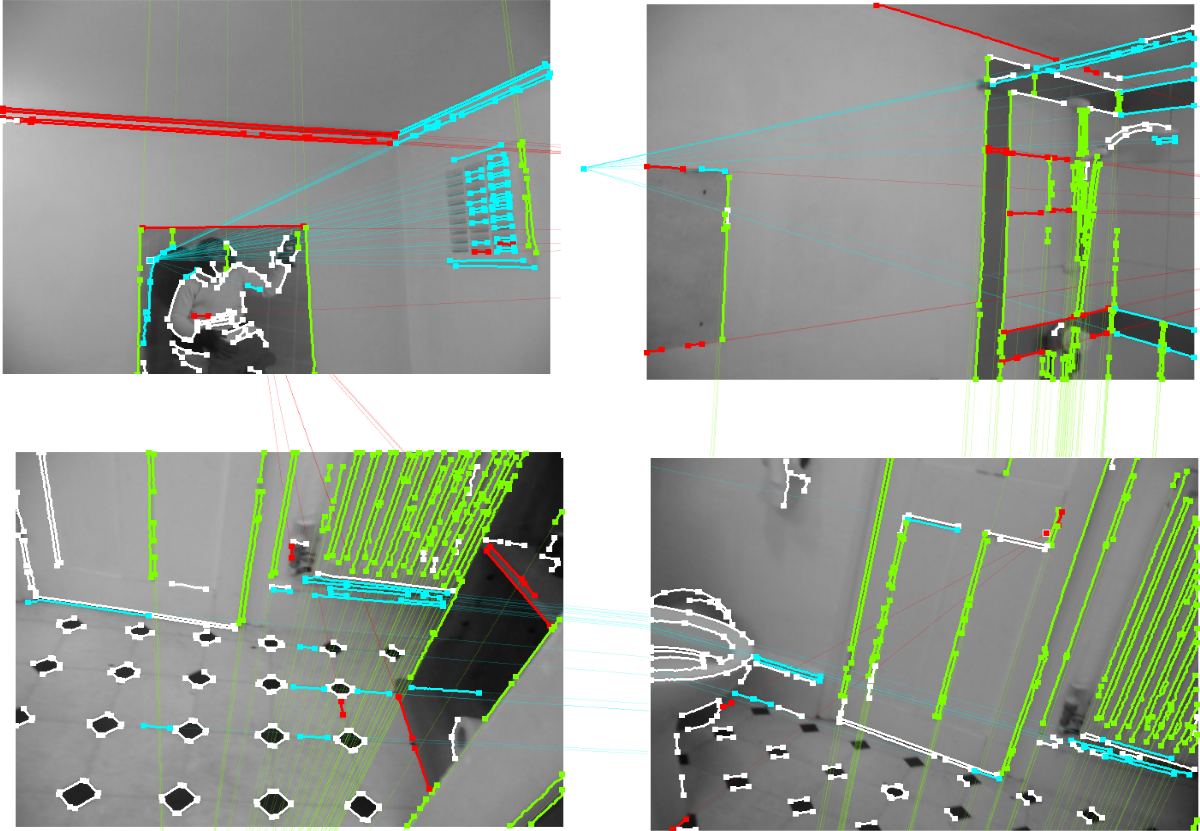
\includegraphics[width=0.5\textwidth]{bathroom_vpts.png}
  \caption{Four frames from the ``bathroom'' sequence and the detected
    vanishing points. The vanishing points are correctly identified
    despite the strong distractor gradients generated by the floor
    tiles, which is possible only by integrating information from
    multiple views into the estimation process. Vertical lines are
    green, horizontal lines are blue (along the room's longer
    dimension) and red (along the room's shorter axis).}
  \label{fig:bathroom-vpts}
\end{figure}

\begin{figure}[tb]
  \centering
      {\bf Single--image estimation}\cite{Zhang02} \hspace{2.25cm}
      {\bf Our method}
  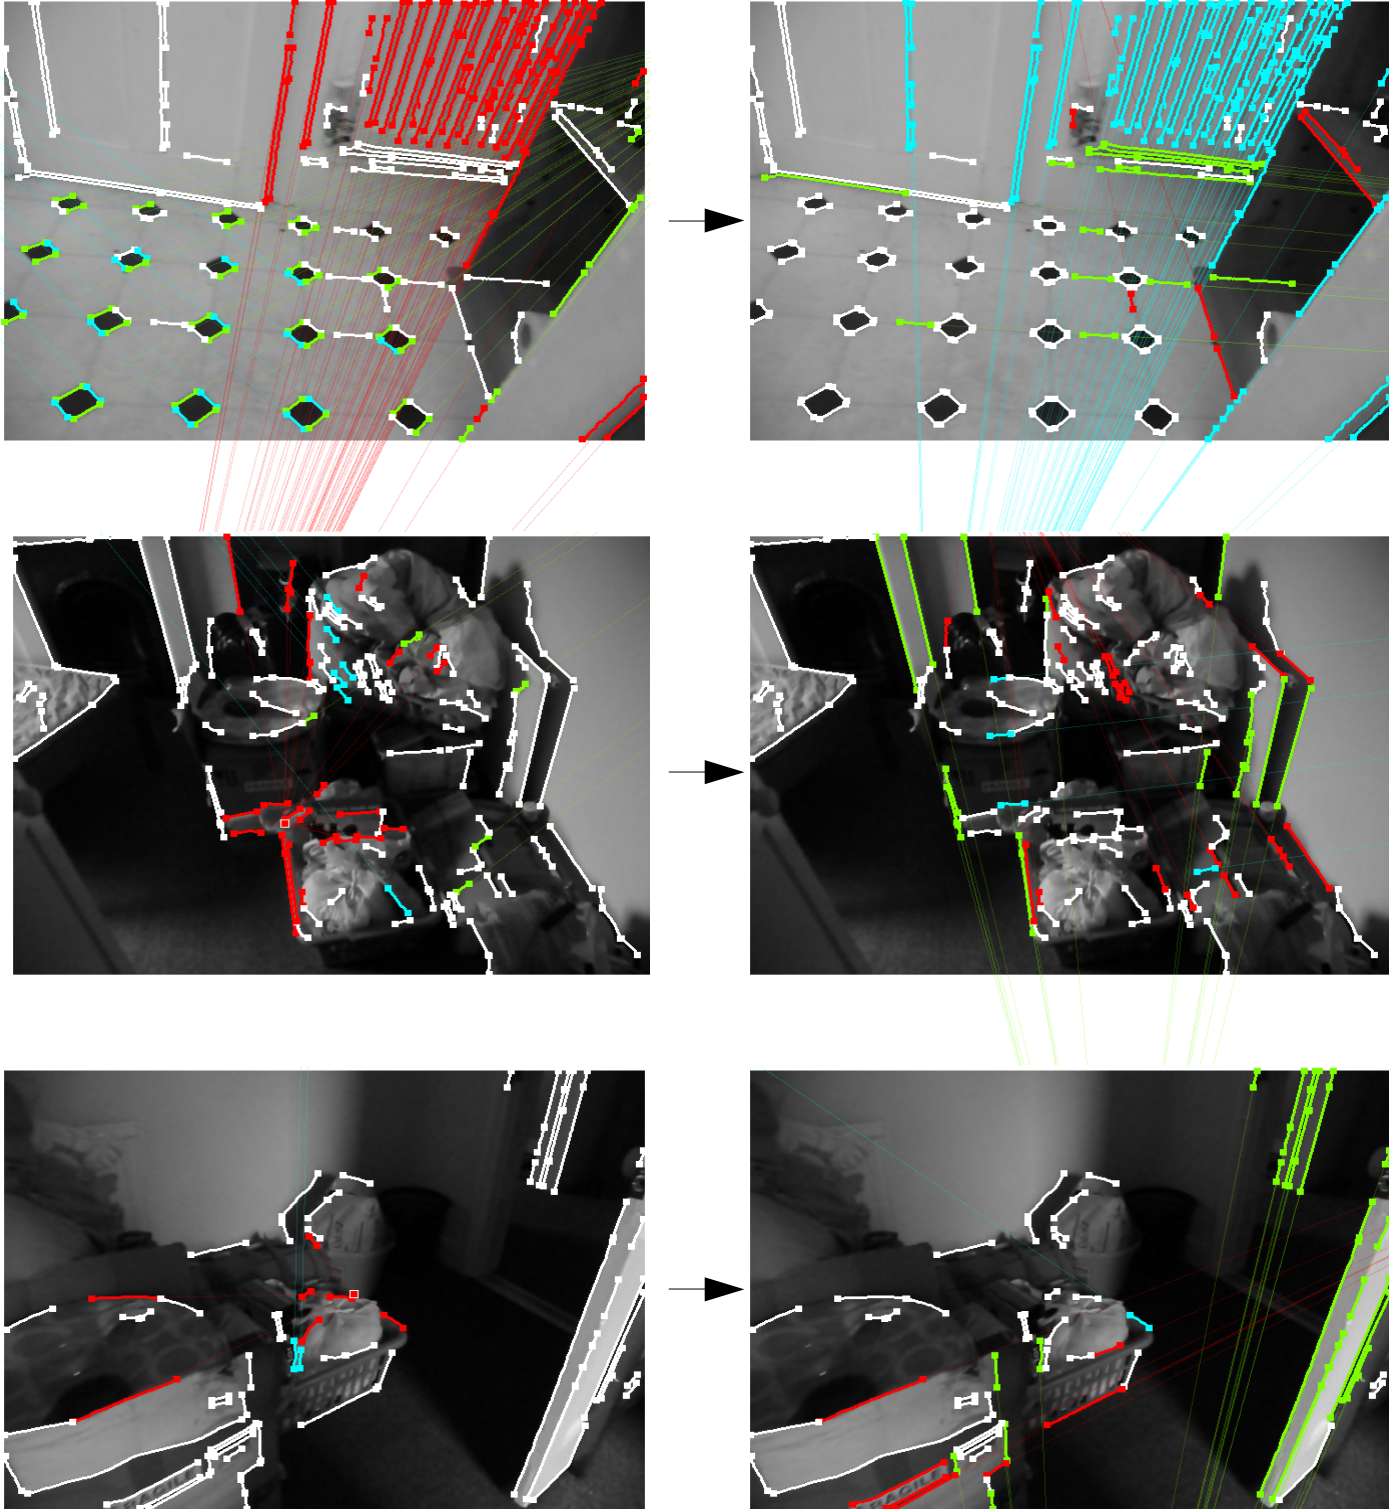
\includegraphics[width=0.5\textwidth]{vpt_comparison.png}
  \caption{Comparison between vanishing points estimated for single
    views (left column) and joint estimates from 20 frames in a video
    sequence (right column). Our method is able to identify vanishing
    directions correctly in these difficult cases, whereas the single
    view estimator is confused by non--Manhattan line segments.}
  \label{fig:vpt-comparison}
\end{figure}

\section{Identifying the vertical direction}
Of the three dominant directions defined by $\SceneR$, two correspond to
horizontal directions and the third to the vertical direction. The
latter is semantically distinct since it defines the orientation of
the ground and ceiling planes, as well as the direction in which
gravity operates. It is easy to identify the vertical axis since
humans necessarily move over the ground plane when capturing video
sequences, and have limited scope for moving the camera in the
up--down direction. We therefore set the vertical axis to that over
which camera positions range the least. Having identified $\SceneR$ there
are only three possible choices, and we found this heuristic to work
correctly in all of our evaluation sequences.


\subsection{Identifying the floor and ceiling planes.}
\label{sect:fcmap}
TODO
An indoor Manhattan scene has exactly one floor and one ceiling plane,
both with normal direction $\vvpt$. It will be useful in the following
sections to have available the mapping $\Hcf$ between the image
locations of ceiling points and the image locations of the floor
points that are vertically below them (see \figref{fcmap}). $\Hcf$ is
a planar homology with axis $\vect{h}=\lvpt\times\rvpt$ and vertex
$\vvpt$ \cite{Criminisi01} and can be recovered given the image
location of any pair of corresponding floor/ceiling points
$(\vect{x_f},\vect{x_c})$ as
\begin{equation}
  \Hcf = I + \mu\frac{\vvpt\vect{h}^T}{\vvpt \cdot \vect{h}} ~,
\end{equation}
where $\mu = \langle\vvpt,\vect{x_c},\vect{x_f},
\vect{x_c}\times\vect{x_f}\times\vect{h}\rangle$ is the characteristic cross
ratio of $\Hcf$.

Although we do not have \textit{a priori} any such pair
$(\vect{x_f},\vect{x_c})$, we can recover $\Hcf$ using the following
RANSAC algorithm. First, we sample one point $\vect{\hat{x}_c}$ from
the region above the horizon in the Canny edge map, then we sample a
second point $\vect{\hat{x}_f}$ collinear with the first and
$\vvpt$ from the region below the horizon. We compute the
hypothesis map $\Hcfhat$ as described above, which we then score by
the number of edge pixels that $\Hcfhat$ maps onto other edge pixels
(according to the Canny edge map). After repeating this for a fixed
number of iterations we return the hypothesis with greatest score.

Many images contain either no view of the floor or no view of the
ceiling. In such cases $\Hcf$ is unimportant since there are no
corresponding points in the image. If the best $\Hcf$ output from the
RANSAC process has a score below a threshold $k_t$ then we set $\mu$
to a large value that will transfer all pixels outside the image
bounds. $\Hcf$ will then have no impact on the estimated model.

\section{Relaxing the Manhattan world assumption}
The strong Manhattan assumption states that any pair of surfaces of
interest are either parallel or orthogonal to one another. One common
deviation from this is scenes with walls that are orthogonal to the
ground and ceiling but not to one another. We define the weak
Manhattan assumption as ``the environment consists of a horizontal
ground plane and corresponding ceiling plane, and a set of vertical
wall segments extending continuously between them.'' Weakly Manhattan
environments contain much of the regularity of strongly Manhattan
environments. We deal with the weak Manhattan assumption as
follows. First, we run the EM algorithm described above to obtain
$\SceneR$. Next, for each line $\LineSeg_j$ marked as spurious by the EM
algorithm we find its intersection with the horizon,
\begin{equation}
  \vect{u}_j = \SceneR^{-T} R_i^{-T} \LineSeg_j \times \ez ~,
\end{equation}
which would be its vanishing point if it were horizontal in the
world. Vertical surfaces of a given orientation will generate
identical $\vect{u}_j$ (modulo measurement error), so we may identify
additional vertical orientations by clustering the intersections
$\{\vect{u}_j\}$. We adopt a voting algorithm in which we parametrise
$\vect{u}_j$ in terms of the angle $\theta_j$ about the $z$ axis
\begin{equation}
  \theta_{j} = \mbox{atan}
  ({\ey}^T\vect{u}_j,~ {\ex}^T\vect{u}_j) ~.
\end{equation}
We accumulate the $\theta_j$ into histogram bins and identify any
local maxima $\theta_i^*$ above a threshold $k$. Each $\theta_i^*$
represents a cluster of line segments corresponding to an additional
vertical orientation. Finally, we re--estimate the vanishing point for
each cluster by minimising the likelihood \eqref{line-lik} via
least--squares.

\section{Guided Line Search}
